\begin{frame}
\frametitle{Планирование потоков}
\begin{itemize}
    \item<1->Планировщик (scheduler) - компонент ОС, который определяет
    \begin{itemize}
        \item<2->когда переключаться с потока;
        \item<3->на какой поток переключаться.
    \end{itemize}
\end{itemize}
\end{frame}

\begin{frame}
\frametitle{Простое планирование}
\begin{itemize}
    \item<1->Рассмотрим простейшую задачу планирования
    \begin{itemize}
        \item<2->все задачи известны заранее;
        \item<3->про каждую задачу известно, сколько времени она займет;
        \item<4->задачи работают без переключений;
        \item<5->т. е. нам осталось только определить порядок.
    \end{itemize}
\end{itemize}
\end{frame}

\begin{frame}
\frametitle{Пропускная способность}
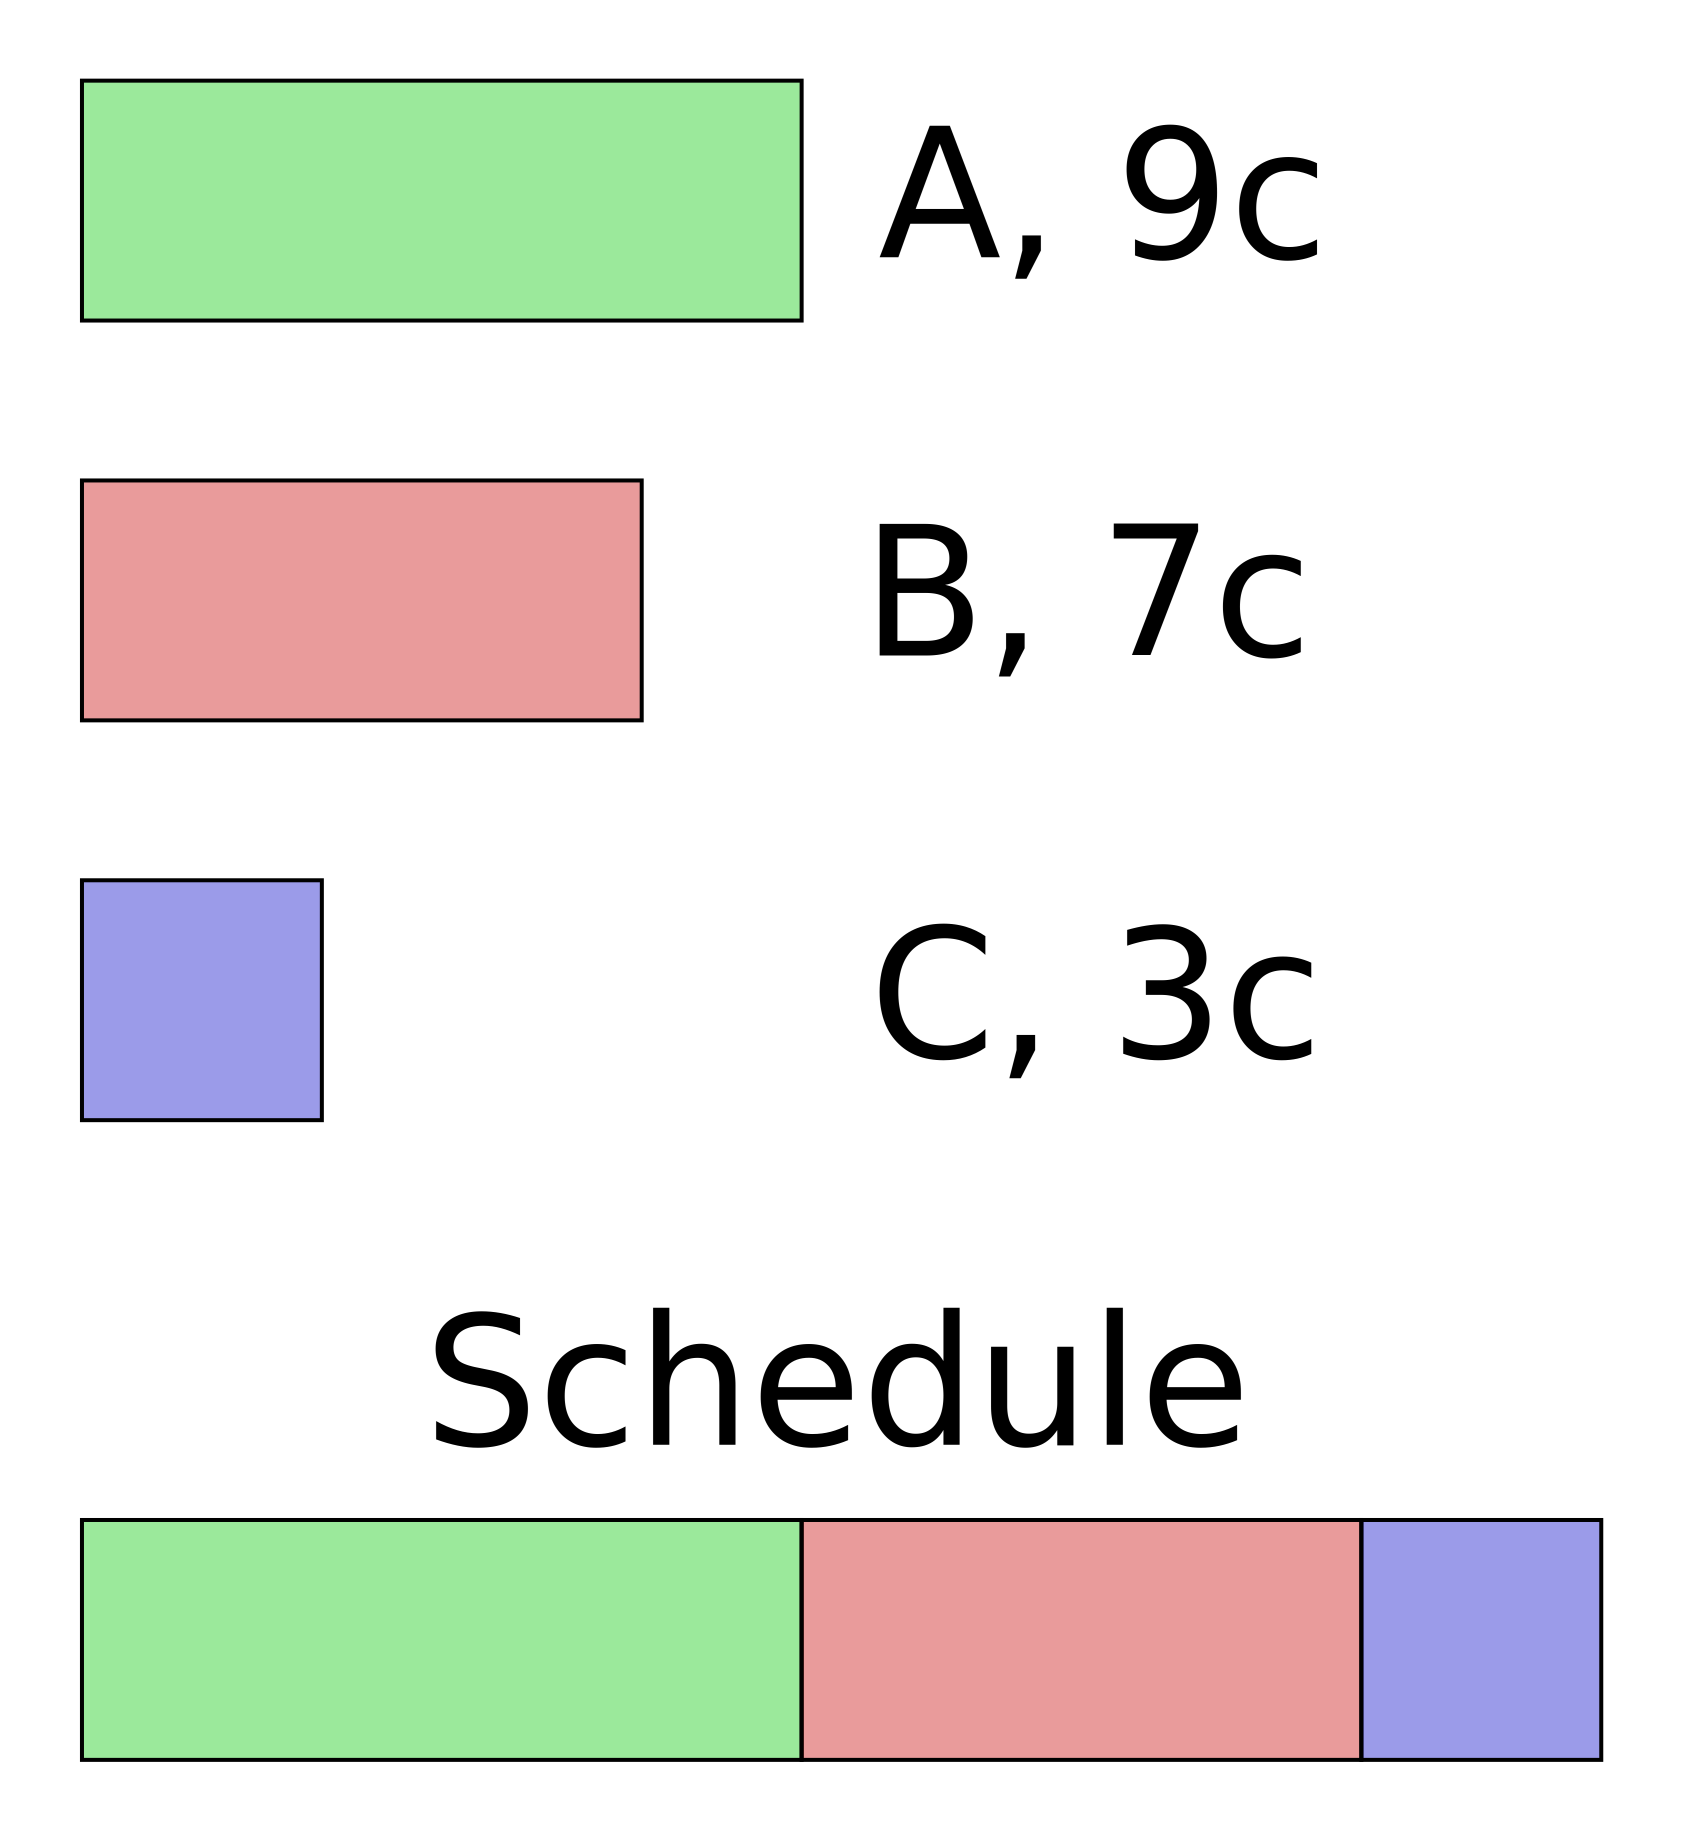
\includegraphics[height=.6\textheight]{sched0}
\end{frame}

\begin{frame}
\frametitle{Пропускная способность}
\includegraphics[height=.6\textheight]{sched1}
\end{frame}

\begin{frame}
\frametitle{Среднее время ожидания}
\begin{itemize}
    \item<1->Пусть все задачи принадлежат разным пользователям
    \begin{itemize}
        \item<2->пользователю важно, сколько ему нужно ждать
             завершения его задачи;
        \item<3->давайте в качестве метрики использовать среднее время ожидания.
    \end{itemize}
\end{itemize}
\end{frame}

\begin{frame}
\frametitle{Среднее время ожидания}
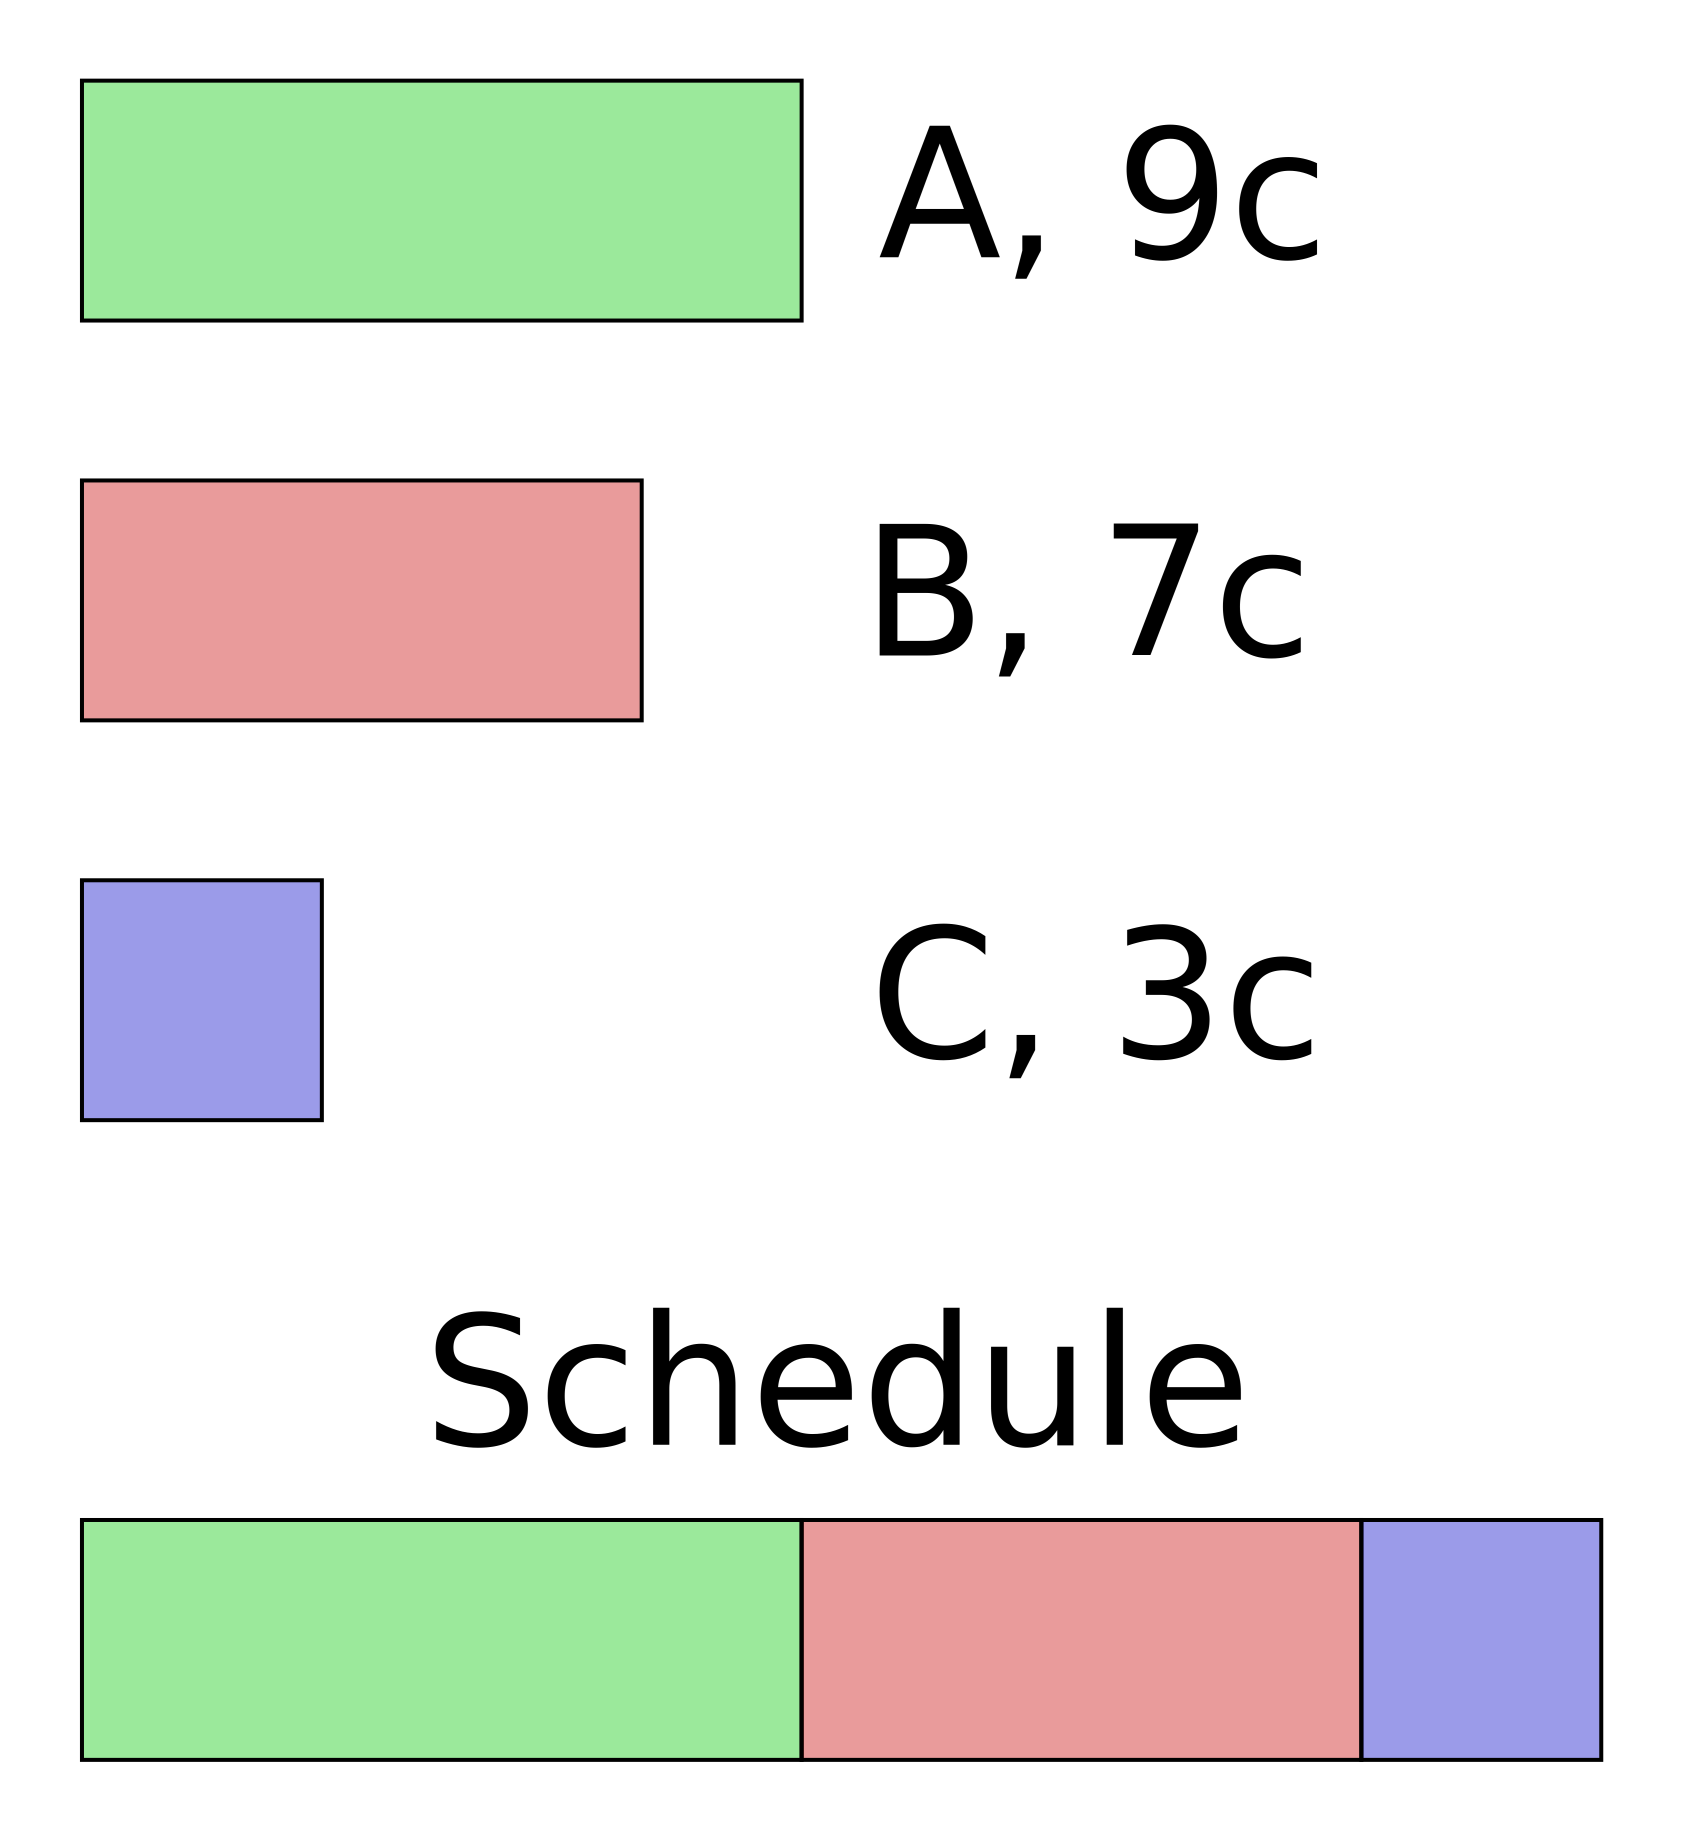
\includegraphics[height=.6\textheight]{sched0}
\end{frame}

\begin{frame}
\frametitle{Среднее время ожидания}
\includegraphics[height=.6\textheight]{sched1}
\end{frame}

\begin{frame}
\frametitle{Динамическое создание задач}
\begin{itemize}
    \item<1->Зачастую все задачи не известны заранее
    \begin{itemize}
        \item<2->задачи могут создаваться в произвольные моменты времени;
        \item<3->каждая вновь появившаяся задача может изменить решение
             планировщика.
    \end{itemize}
\end{itemize}
\end{frame}

\begin{frame}
\frametitle{IO операции}
\begin{itemize}
    \item<1->Задачи могут давать команды устройствам или ждать каких-то событий:
    \begin{itemize}
        \item<2->запись/чтение на/с HDD (порядка нескольких мс);
        \item<3->ждать входящих соединений по сети;
        \item<4->ждать, пока пользователь нажмет на клавишу.
    \end{itemize}
\end{itemize}
\end{frame}

\begin{frame}
\frametitle{IO операции}
\begin{itemize}
    \item<1->Пока задача ждет завершения IO операции, можно забрать у нее CPU
    \begin{itemize}
        \item<2->время ожидания может быть большим (1мс - очень много для CPU);
        \item<3->утилизация CPU - сколько времени CPU делал полезную работу.
    \end{itemize}
\end{itemize}
\end{frame}

\begin{frame}
\frametitle{Утилизация}
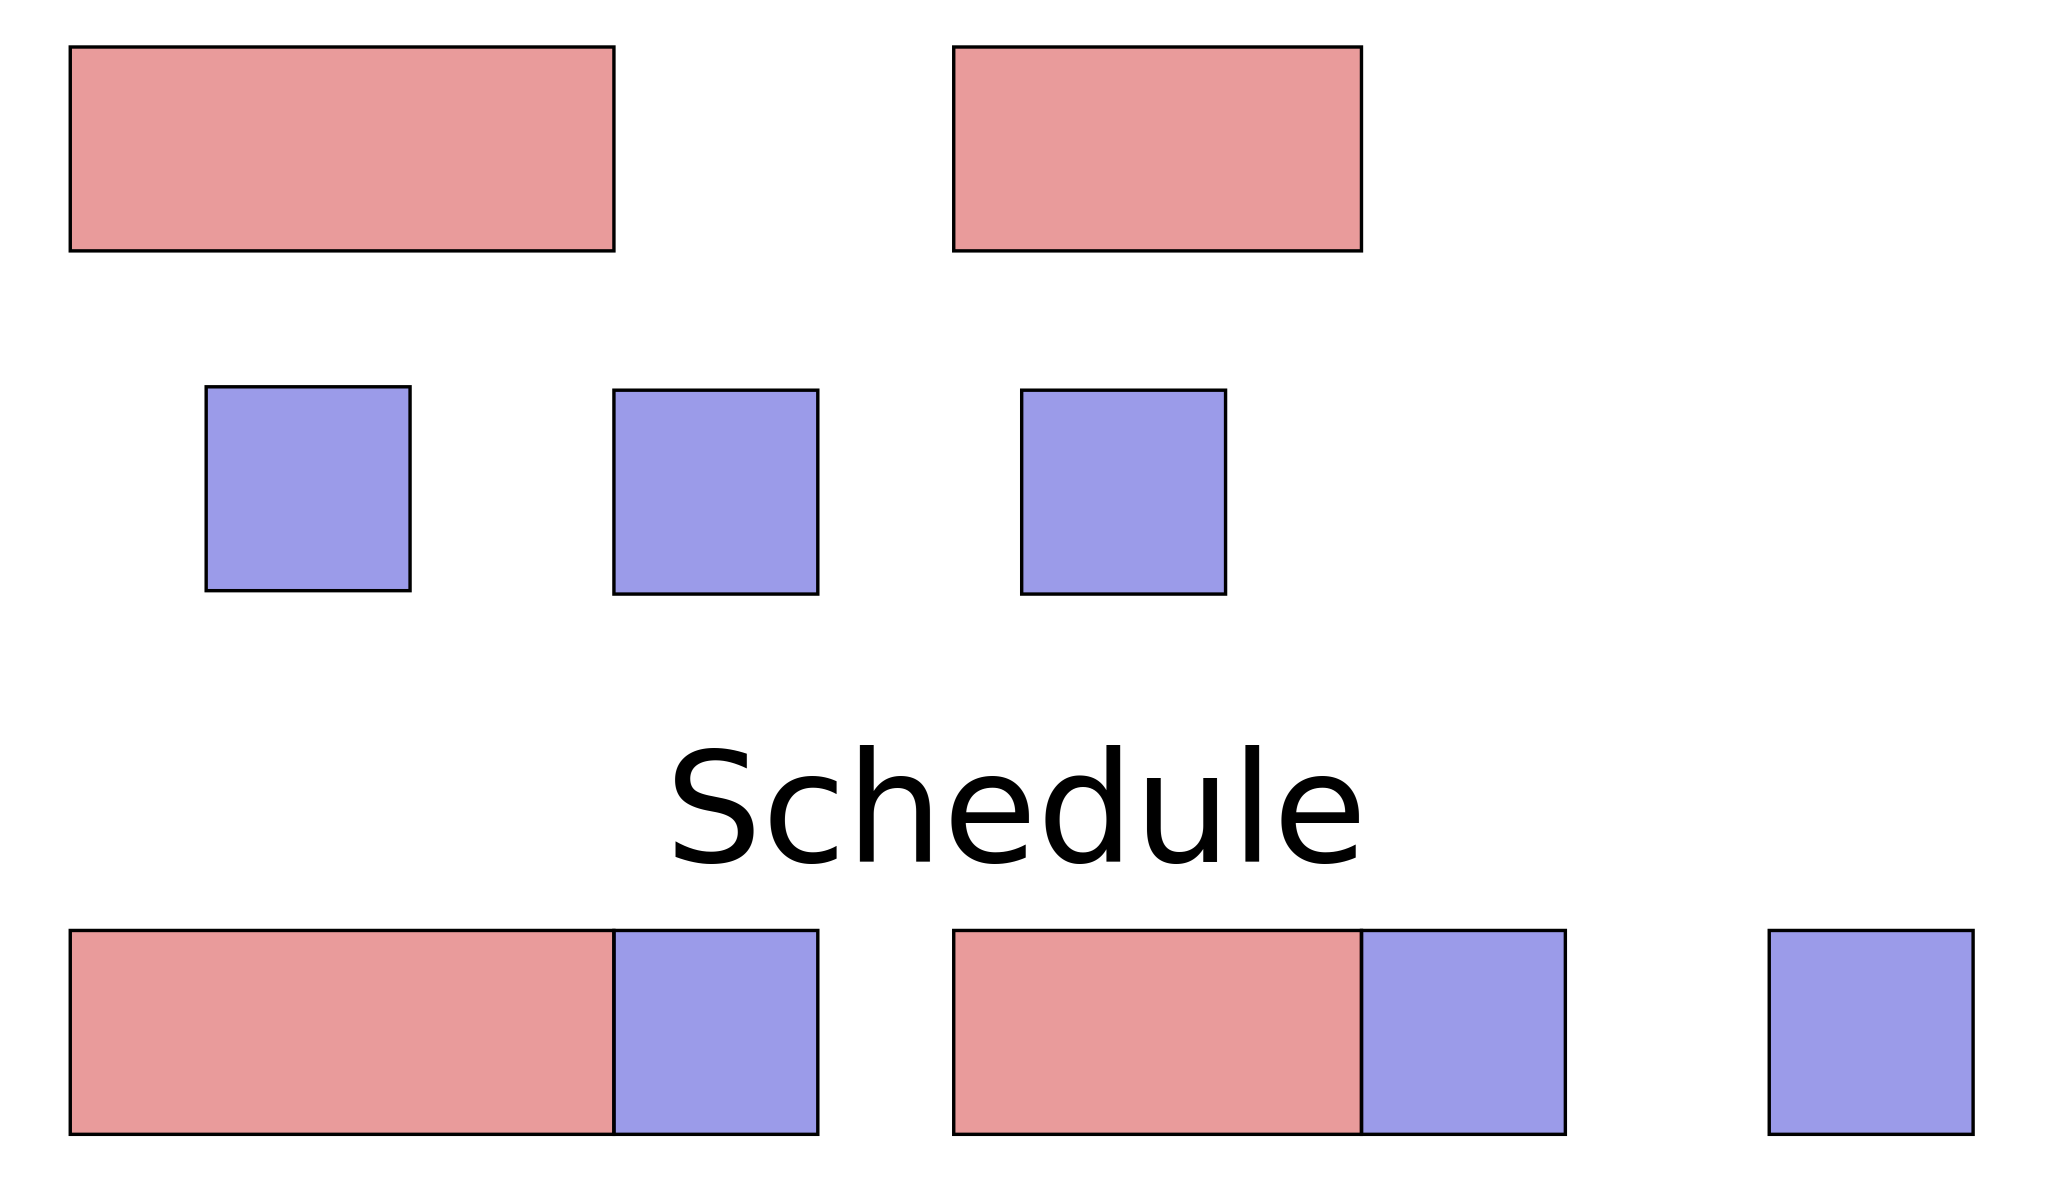
\includegraphics[height=.5\textheight]{sched2}
\end{frame}

\begin{frame}
\frametitle{Утилизация}
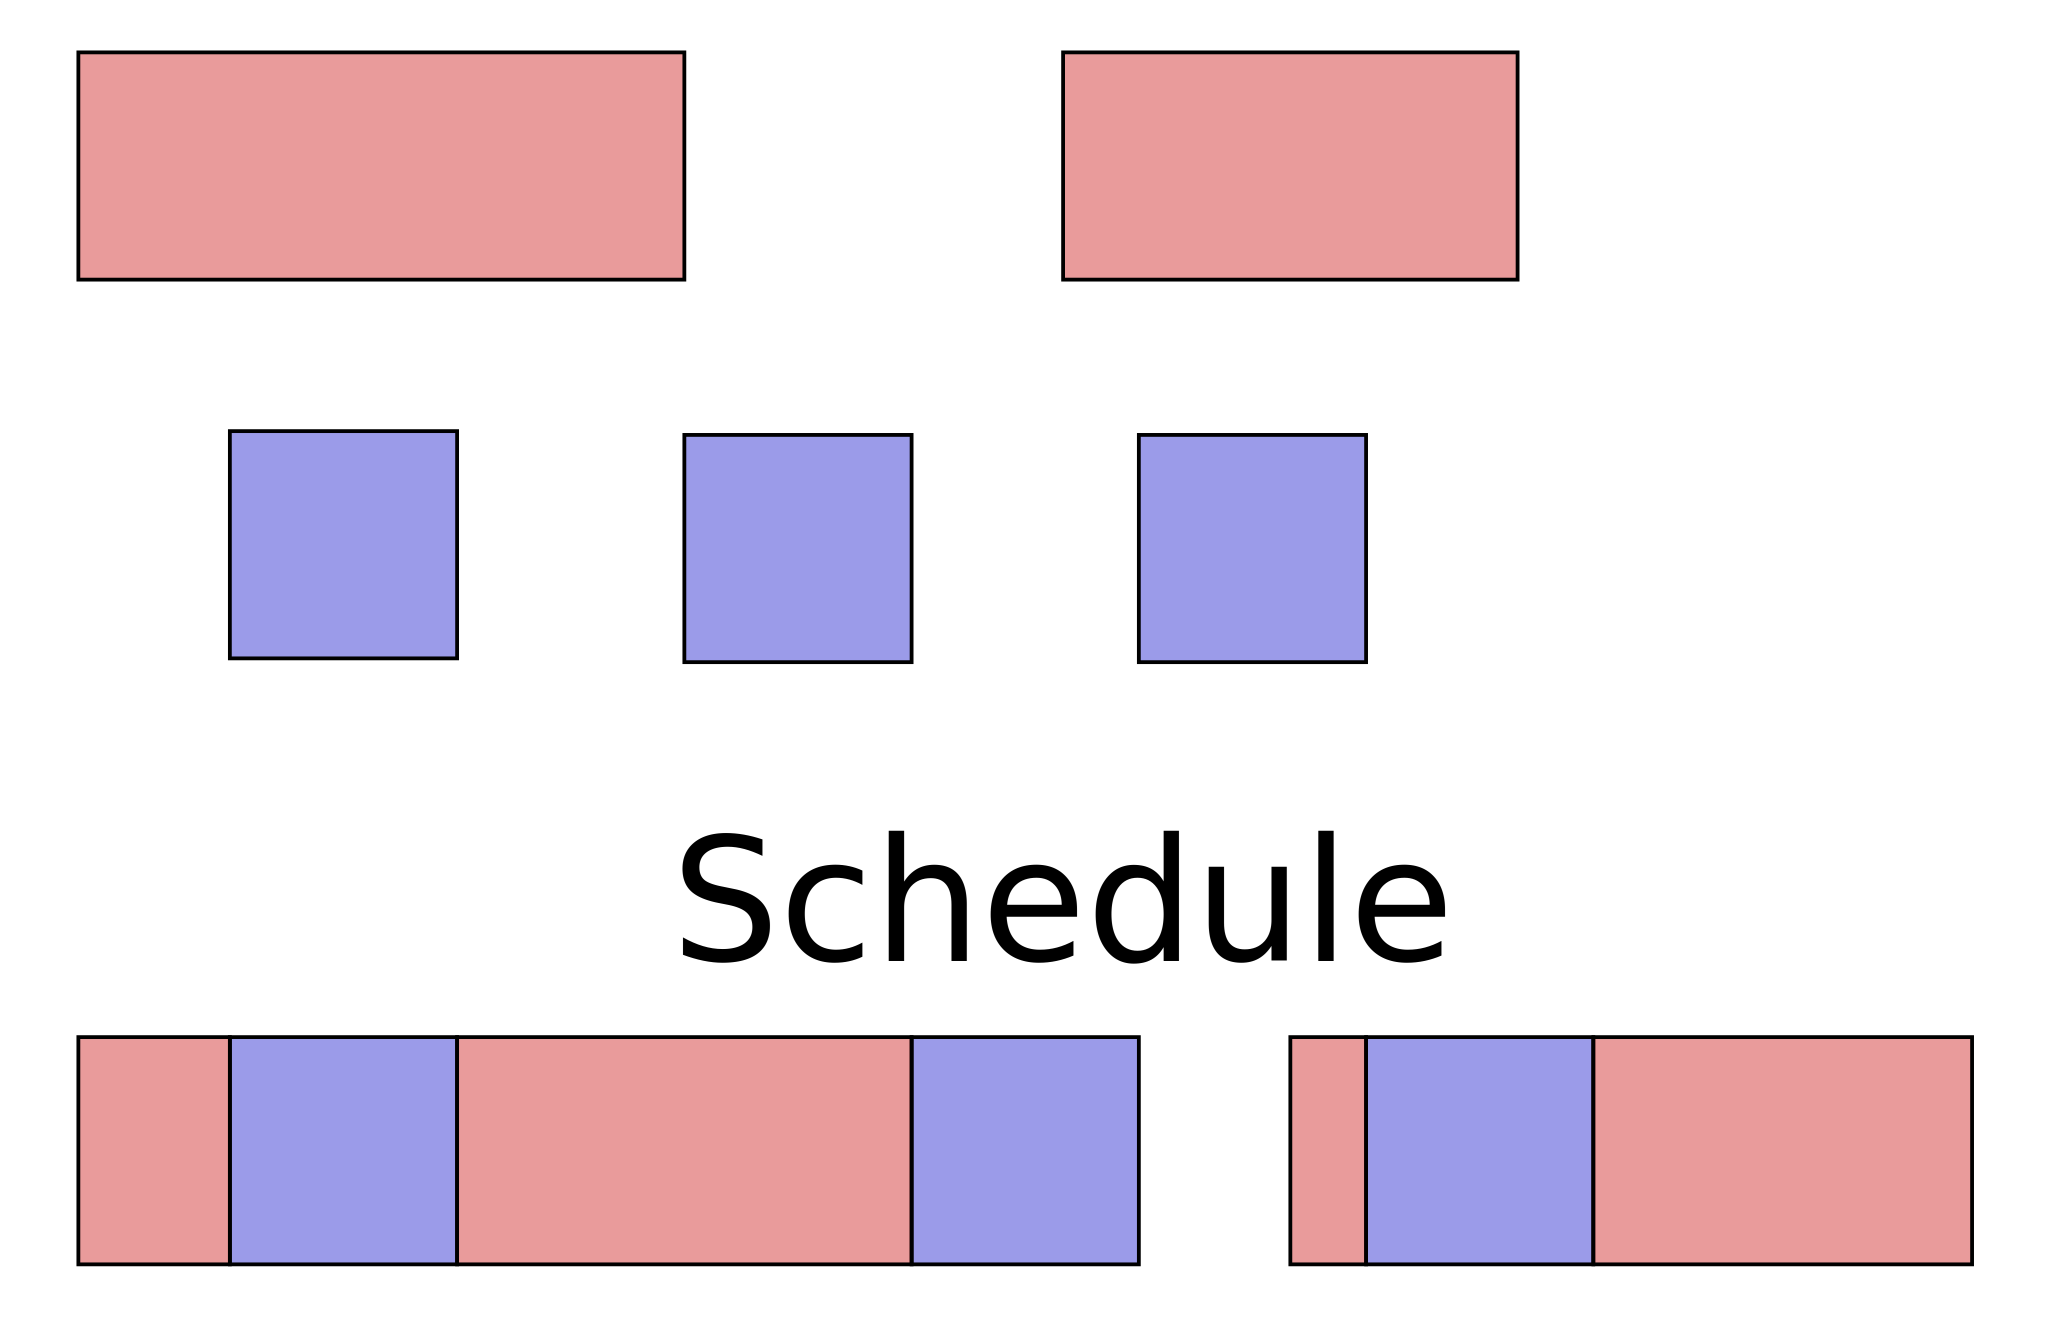
\includegraphics[height=.5\textheight]{sched3}
\end{frame}

\begin{frame}
\frametitle{Информация о задаче}
\begin{itemize}
    \item<1->Зачастую время работы задачи и расписание ее IO не известны
    \begin{itemize}
        \item<2->задачи могут влиять друг на друга или зависеть от внешних
             обстоятельств;
        \item<3->мы можем оценивать эти параметры и классифицировать задачи.
    \end{itemize}
\end{itemize}
\end{frame}

\begin{frame}
\frametitle{IO-bounded и CPU-bounded}
\begin{itemize}
    \item<1->IO-bounded задачи - много IO, но мало вычислений:
    \begin{itemize}
        \item<2->например, текстовый редактор;
        \item<2->вообще приложения, ожидающие ввода пользователя.
    \end{itemize}
    \item<3->CPU-bounded задачи - много вычислений, но мало IO:
    \begin{itemize}
        \item<4->например, научные вычисления;
        \item<4->компиляция программ.
    \end{itemize}
\end{itemize}
\end{frame}

\begin{frame}
\frametitle{Round Robin}
\begin{itemize}
    \item<1->Round Robin - выдаем потокам квант времени на CPU по очереди:
    \begin{itemize}
        \item<2->поток, отработавший свой квант, встает в конец очереди;
        \item<3->каждый новый поток встает в конец очереди;
        \item<4->потоки, дождавшиеся завершения IO, встают в конец очереди;
        \item<5->CPU отдается потоку в начале очереди.
    \end{itemize}
\end{itemize}
\end{frame}

\begin{frame}
\frametitle{Достоинства Round Robin}
\begin{itemize}
    \item<1->К списку достоинств Round Robin можно отнести:
    \begin{itemize}
        \item<2->подход очень прост;
        \item<3->время ожидания CPU ограничено - никто не голодает.
    \end{itemize}
\end{itemize}
\end{frame}

\begin{frame}
\frametitle{Round Robin}
\includegraphics[height=.4\textheight]{rr0}
\end{frame}

\begin{frame}
\frametitle{Round Robin}
\includegraphics[height=.4\textheight]{rr1}
\end{frame}

\begin{frame}
\frametitle{Round Robin}
\includegraphics[height=.4\textheight]{rr2}
\end{frame}

\begin{frame}
\frametitle{Round Robin}
\includegraphics[height=.4\textheight]{rr3}
\end{frame}

\begin{frame}
\frametitle{Round Robin}
\includegraphics[height=.4\textheight]{rr4}
\end{frame}

\begin{frame}
\frametitle{Round Robin}
\includegraphics[height=.4\textheight]{rr5}
\end{frame}

\begin{frame}
\frametitle{Round Robin}
\includegraphics[height=.4\textheight]{rr6}
\end{frame}

\begin{frame}
\frametitle{Round Robin}
\includegraphics[height=.4\textheight]{rr7}
\end{frame}

\begin{frame}
\frametitle{Round Robin}
\includegraphics[height=.4\textheight]{rr8}
\end{frame}

\begin{frame}
\frametitle{Round Robin}
\includegraphics[height=.4\textheight]{rr9}
\end{frame}

\begin{frame}
\frametitle{Round Robin}
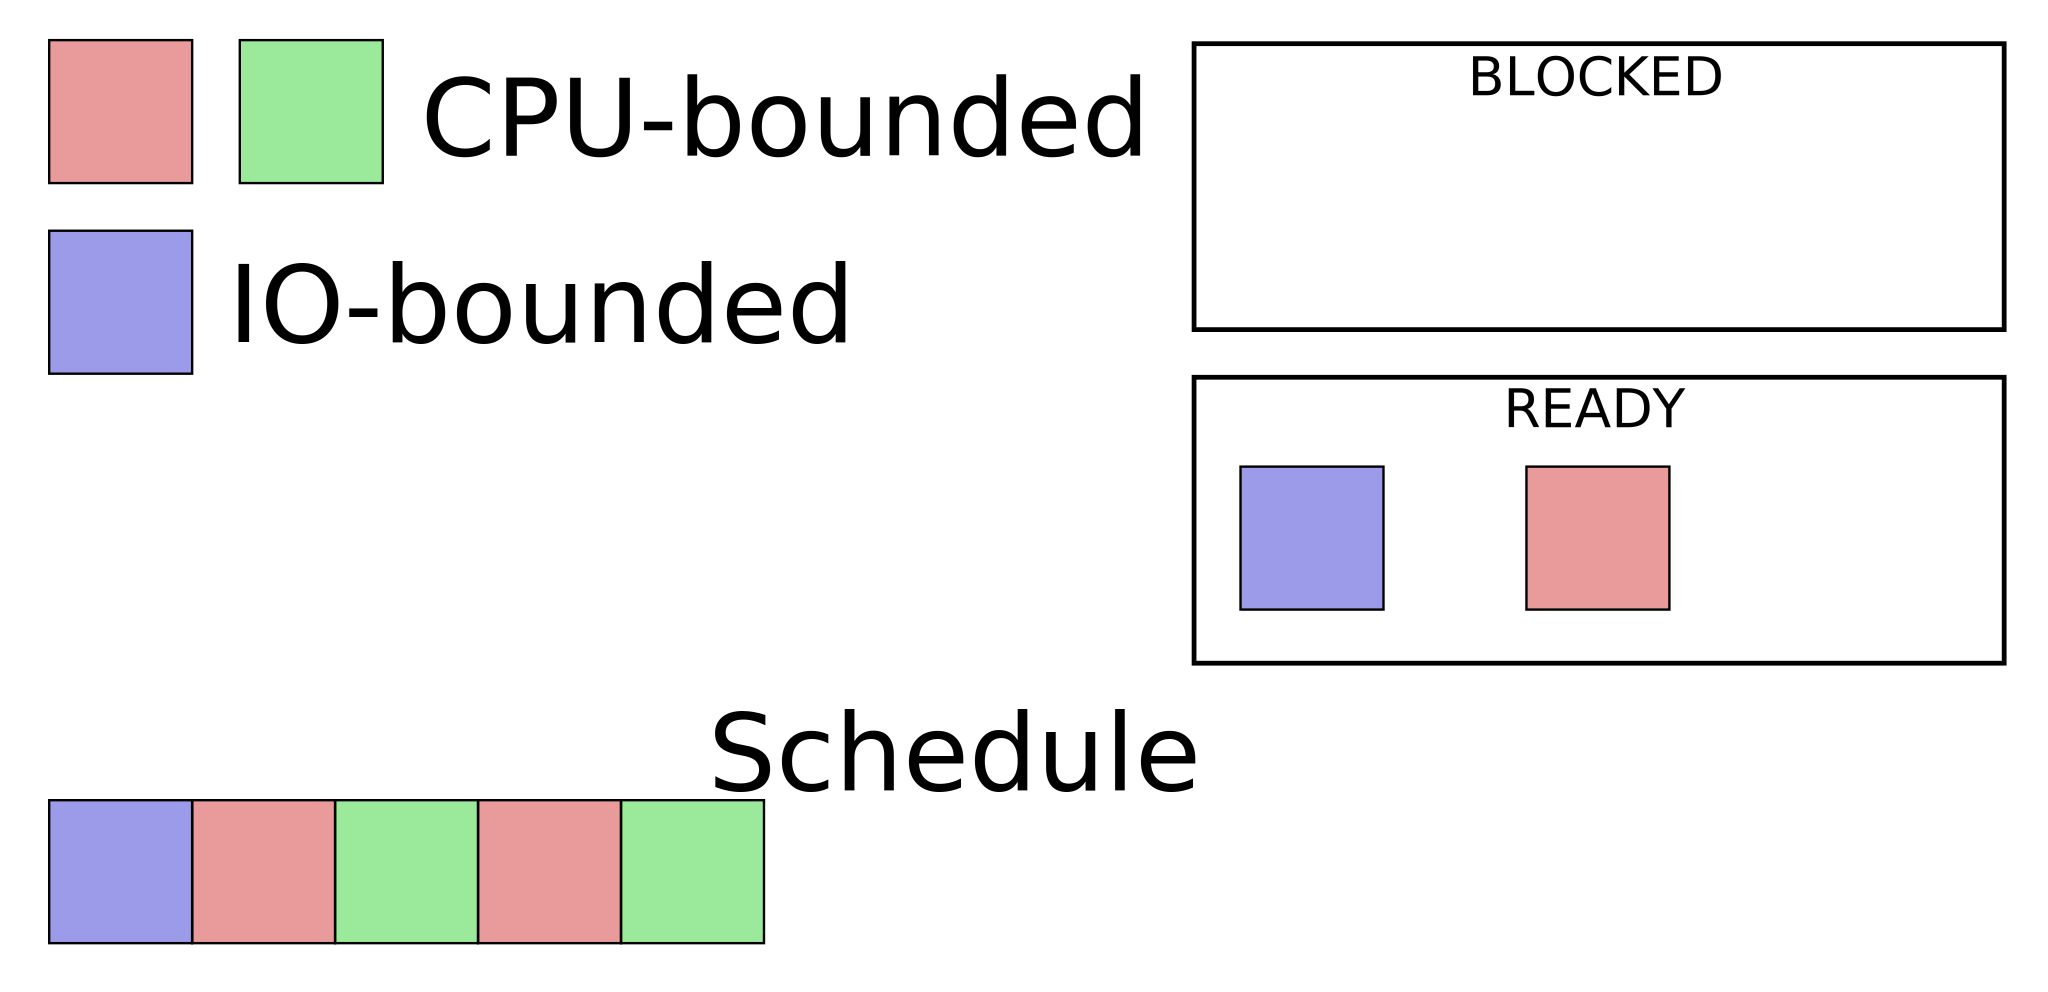
\includegraphics[height=.4\textheight]{rr10}
\end{frame}

\begin{frame}
\frametitle{Round Robin}
\includegraphics[height=.4\textheight]{rr11}
\end{frame}

\begin{frame}
\frametitle{Round Robin}
\includegraphics[height=.4\textheight]{rr12}
\end{frame}

\begin{frame}
\frametitle{Round Robin}
\includegraphics[height=.4\textheight]{rr13}
\end{frame}

\begin{frame}
\frametitle{Round Robin}
\includegraphics[height=.4\textheight]{rr14}
\end{frame}

\begin{frame}
\frametitle{Round Robin}
\includegraphics[height=.4\textheight]{rr15}
\end{frame}

\begin{frame}
\frametitle{Round Robin}
\includegraphics[height=.4\textheight]{rr16}
\end{frame}

\begin{frame}
\frametitle{Round Robin}
\includegraphics[height=.4\textheight]{rr17}
\end{frame}

\begin{frame}
\frametitle{Round Robin}
\includegraphics[height=.4\textheight]{rr19}
\end{frame}

\begin{frame}
\frametitle{Round Robin}
\includegraphics[height=.4\textheight]{rr20}
\end{frame}

\begin{frame}
\frametitle{Round Robin}
\includegraphics[height=.4\textheight]{rr21}
\end{frame}

\begin{frame}
\frametitle{Round Robin}
\includegraphics[height=.4\textheight]{rr22}
\end{frame}

\begin{frame}
\frametitle{Round Robin}
\includegraphics[height=.4\textheight]{rr23}
\end{frame}

\begin{frame}
\frametitle{Round Robin}
\includegraphics[height=.4\textheight]{rr24}
\end{frame}

\begin{frame}
\frametitle{Round Robin}
\includegraphics[height=.4\textheight]{rr25}
\end{frame}

\begin{frame}
\frametitle{Round Robin}
\includegraphics[height=.4\textheight]{rr26}
\end{frame}

\begin{frame}
\frametitle{Round Robin}
\includegraphics[height=.4\textheight]{rr27}
\end{frame}

\begin{frame}
\frametitle{Выбор кванта времени}
\begin{itemize}
    \item<1->Из каких соображений стоит выбирать квант времени?
    \begin{itemize}
        \item<2->чем больше квант
        \begin{itemize}
            \item<3->тем меньше доля времени на переключение;
            \item<3->тем больше время отклика;
        \end{itemize}
        \item<4->чем меньше квант
        \begin{itemize}
            \item<5->тем больше доля времени на переключение;
            \item<5->тем меньше время отклика.
        \end{itemize}
    \end{itemize}
\end{itemize}
\end{frame}

\begin{frame}
\frametitle{Выбор кванта времени}
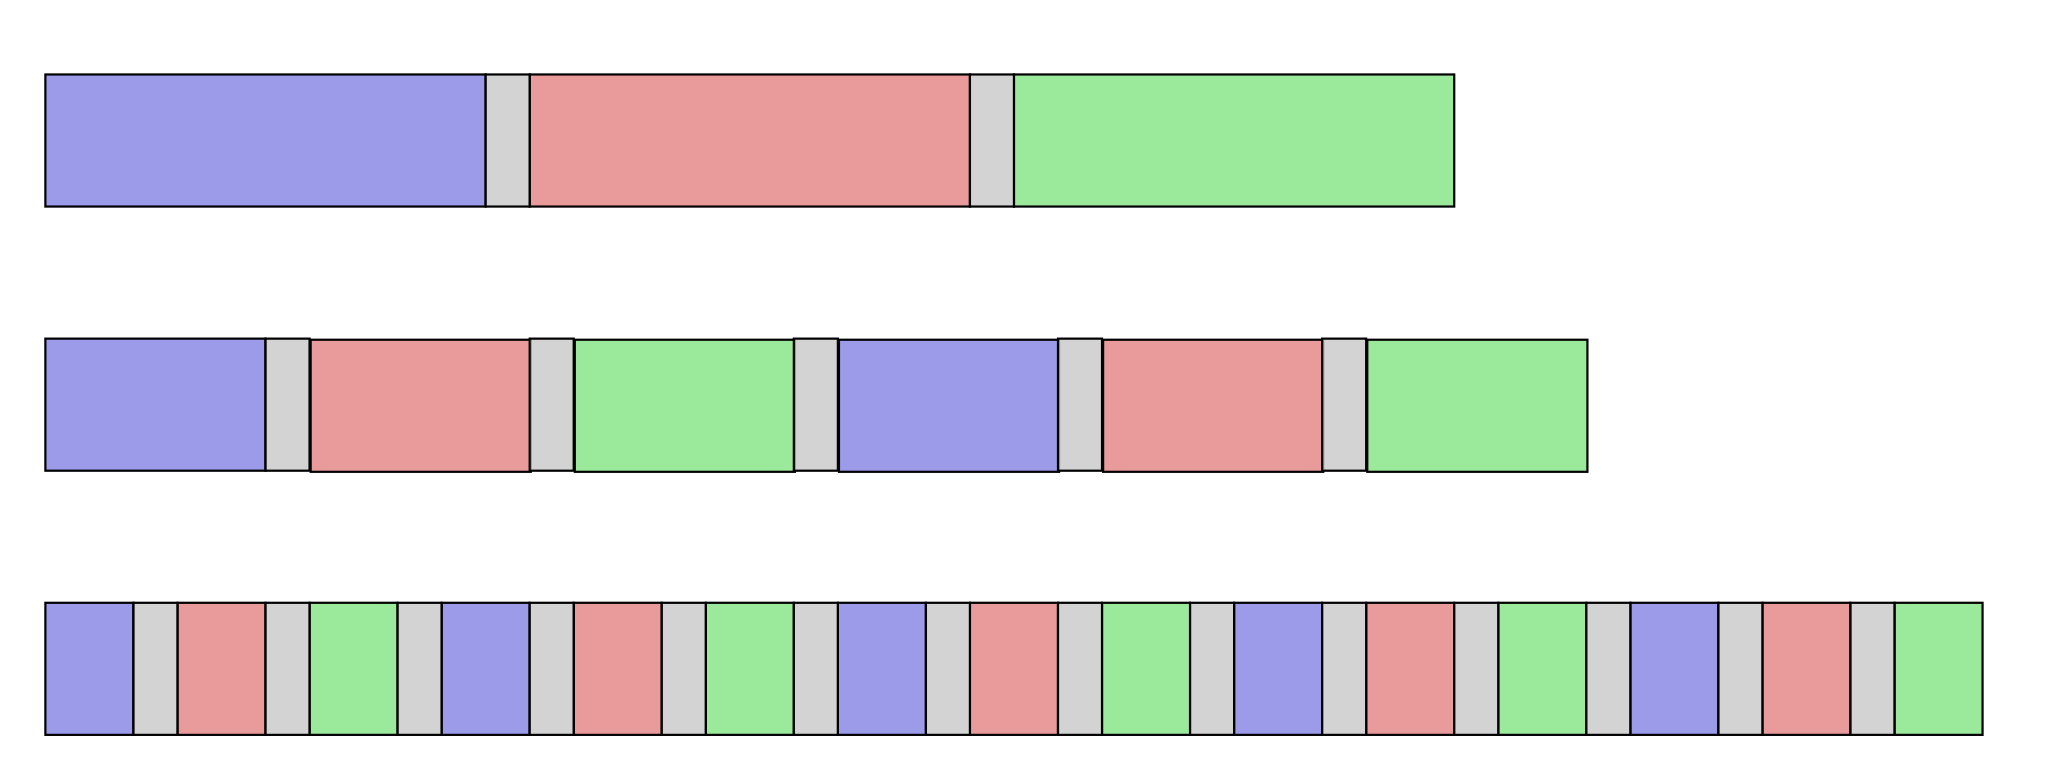
\includegraphics[height=.3\textheight]{multithreading}
\end{frame}
